\subsection{Design}

As one of the selection of high-interaction malware scanning
methods available for use in the malucrawl framework,
Capture-HPC\cite{capture-hpc} is a way of
realistically emulating a user browsing to a given URL in a real web browser.
Capture-HPC is designed as a client honeypot, where in contrast to the usual and
more common form of passive honeypots that simply wait for incoming attacks,
goes out and requests content from the Internet and attempts to detect any
malicious actions performed by the content. Capture-HPC was developed at Victoria
University in Wellington NZ and is maintained be the HoneyNet project\cite{honeynet}.

\subsubsection{Capture-HPC in Detail}

Capture-HPC uses virtualisation to simulate user browsing, using a web browser
running in a monitored and externally controlled Virtual Machine. There are two
distinct pieces of software used to do this, a client to run the web browser on
the virtual machine and monitor for malicious activity, and a server to
orchestrate URL scanning between however many clients are being used and to
reset client VMs when malicious activity is detected. The client and server
components communicate over a network connection.
\paragraph{The Client}
The Capture-HPC client is a C++ program that runs on Windows XP, Vista, or 7.
Its role is to automatically download content from the internet and to monitor
the VM for any
suspicious activity, reporting the outcome rendering URLs to the server. The
client is capable of driving a number of applications using URLS, from web
browsers such as Microsoft Internet Explorer and Mozilla Firefox, to downloading and opening
Microsoft Word documents and Adobe PDFs. For the purposes of the project, the
use of Internet Explorer is prioritised as a starting point for malware scanning
that can be easily extended to cover the other applications. To detect any
malicious activity that may be caused by visiting a website, or opening a
downloaded file, a collection of kernel drivers are used. The kernel drivers
watch filesystem, network and process activity at a low level inside the
operating system, ensuring that
unusual activity can be detected despite attempts from any malware to conceal
its actions. This isn't a technique that works in general on a PC where the user
may be performing any number of other actions whilst using the machine, but
works well in the controlled environment provided by the virtual machine. To
stop the small number of standard processes and filesystem changes made during
normal operation of the operating system and client applications triggering the
malware detection, Capture-HPC uses a set of "exclusion lists" that specify
actions for each monitoring tool that should be considered as safe. It is also
possible to specify precisely which actions should cause the monitoring tool to
report suspected malicious activity.
\paragraph{The Server}
The Capture-HPC server program that controls the clients is a Java program that
will run on most platforms (platform compatibility is limited by the VM revert
script detailed below). The role of the server is to communicate the exclusion
lists and URLs to be tested to the clients, and then collect the results of the
analysis. The server also uses an external script to reset the virtual machine
if malicious activity is detected by the client. The server also resets the
client if it does not respond to keepalive packets, so the client does not get
stuck on a URL that errors or a very large file such as a DVD. There exists two
options for supplying URLs to the
Capture-HPC server, using a plaintext input file with one URL on each line (the
line can also contain options controlling which client application is used to
open the URL) or a MySQL database with a schema provided with the application.
The server stores the results in text files labelled for safe URLs, URLs that
cause an error, dangerous URLS and the current
progress by default, with additional detail for suspicious URLs stored in a file
with the name of the suspicious URL (URL encoded). This is not ideal for use within
the project, but fortunately Capture-HPC will store all results in the
relational database if one is configured. URLs can be inserted into the
database, and when the server is run, the URLs are annotated with the results of
the scanning, with additional detail stored in other tables.
The use of a MySQL table for a queue
could be considered an anti-pattern as discussed in \cite{anti-queue}, but is the best of
the options available for providing Capture-HPC with data, and retrieving the
results, presenting an easiliy accessible interface for framework components to
integrate with wither locally or remotely. Unfortunately the Capture-HPC server
also has to be restarted to
consume new URLs from the database, with any finished URLs that are left in the
database processed again. The Capture-HPC server is configured using an XML
configuration file.
\paragraph{VM Integration}
The version of Capture-HPC to be used in the project supports VMware as its
virtualisation platform, and the ECS VM infrastructure also runs on VMware
products. Most VMWare products offer an API for programmatically interacting
with the Virtual Machines being hosted, known as VIX, and Capture-HPC uses this
API to reset VMs that detect any suspicous activity. The API however only has
bindings in perl and C,
so a bridging program written in C is supplied with Capture-HPC and must be
compiled independently of the server. Each virtual machine being used as a
Capture-HPC client needs to have the client software installed, and then a
snapshot taken. A VM Snapshot is a method of backing up the VM in manner that
preserves all information about the state of the VM, including the memory,
meaning that the state of the machine can quickly be restored to its original
after a malware detection. The bridging utility simply reverts the VM to the
first snapshot it can find, and then re-starts the Capture-HPC client. The
separation of the VM API component from the rest of the server proved to be
usefil in the project, as some modifications needed to be made to how VMs are
reverted, as detailed below.

\subsubsection{How Capture-HPC is used in the project}

Capture-HPC is the most accurate simulation of user browsing used by the project
as a malware scanner, and has a very low URL throughput thanks to each URL
needing to be rendered in a web browser. The throughput is further reduced 
the need to revert the VM every time malicious activity is detected. Therefore
it is necessary to limit the number of URLs that Capture-HPC is required to
process. As discussed previously, limiting of the URLs processed by the
high-interaciton malware scanners 
is done by a classification system, and only URLS that are strongly suspected to
harbour malware are submitted for scanning. In addition to the confidence factor
that each malware analyser in the framework must return, Capture-HPC is also
capable of returning a description of the actions taken by a malicious page, and
these details are returned to the framework for optional in-depth analysis. It
is also possible to calculate the ideal confidence value for a given classifier
and set of malware analysers working alongside Capture-HPC so that an optimal
set of URLs provided for time versus detection rate.

\subsubsection{Security Considerations}

As Capture-HPC renders web pages, there is a significant risk that any malicious
content will take over the client VM and try to exploit any other computers
connected to the VM or abuse resources in other ways such as sending spam.
To mitigate this threat, a set of preventative measures are taken. 
Figure \ref{fig:sec-1} shows the architectures used for the implementation of the security
considerations.

\begin{figure}[htb]
\centering
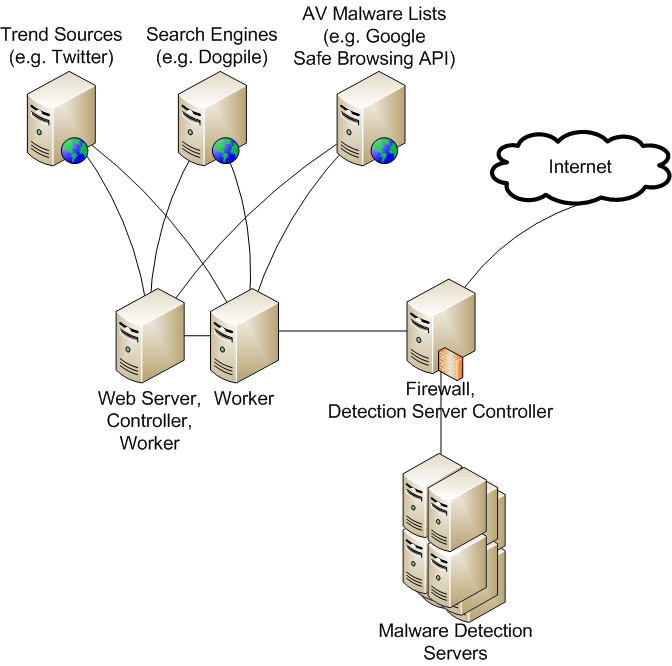
\includegraphics[width=0.8\textwidth]{img/physical-arch-pres.png}
\caption{Secure Architecture}
\label{fig:sec-1}
\end{figure}

To secure the virtual machine(s) running the Capture-HPC client, a Linux
firewall is placed between the VMs and the network, with the client VMs only
able to communicate with the outside network via the firewall. The firewall
blocks all ports by default, only proxying a small selection of ports and
forwarding no ports. To allow the Capture-HPC client to resolve URLs to IP
addressed, DNS
queries are proxied through the firewall, with all requests logged. All HTTP and
HTTPS requests are also proxied and logged using a weekly/monthly rolling log
so that any suspicious
activity can be investigated. A self-signed SSL certificate will be installed on
the client VMs so that HTTPS connections still appear valid despite interception.
A small selection of ports will also be open into and out of the firewall to
allow control of Capture-HPC and reporting of results, and to allow the
Capture-HPC server to communicate with the Capture-HPC clients.

\subsection{Implementation}

\subsubsection{Deployment of Secure Architecture In ECS}

%TODO: compiling client was difficult, but can port image to other platforms,
%re-use capture binary

When deploying Capture-HPC in ECS to form part of our prototype deployment of
the framework, a small group of VMs were used to host the security architecture
discussed above. The gateway VM used Red Hat Enterprise Linux 6 for its
stability and security,
with iptables used to provide a firewall. Squid was used as a HTTP and HTTPS proxy, compiled with
support for dynamically generating certificates for HTTPS websites. To reduce
the amount of effort needed to manually configure the firewall to allow/disallow
different types of traffic during
development of the system, a small tool was written to allow a number of
iptables "profiles" to be created, and then changed using a small shell script. Profiles were written for
development mode with little to no firewall restrictions but with NAT and
forwarding enabled, maintenance mode with restricted ports but forwarding with
NAT instead of proxying, and full mode with proxying and the minimum number of
open ports. The Capture-HPC Server program was also compiled and run from this machine.

The Capture-HPC client was compiled on a Windows XP development VM, and then
deployed to a clean install of Windows XP. Due to the complexity of compiling
the binaries, the installer generated in the build process is included with the
accompanying data package, but would unfortunately still need to be rebuilt for
use on versions of Windows other than XP. It is possible to run the
Capture-HPC client on a Windows Vista or Window 7 install, but was not tested in
the prototype deployment due to time constraints. The Windows XP install used
for the client had no anti-virus or firewall configured, with Internet Explorer
6 installed to present an easy target for malicious sites.

\subsubsection{ECS Specific Customisations}

The specific network architecture meant that some customisations had to be made
to the standard deployment, and to further reduce risk of malware escaping from
behind the firewall. The ECS VM infrastructure uses VMware vSphere to manage its
ESXi VM servers, and the Capture-HPC server must connect to the vSphere
administration console to revert the VMs when malicious activity is detected.
The VM administration API requires authentication, which uses ECS domain
credentials. The consequence of this is that a domain password must be stored in
a file on the VM running the Capture-HPC server, which has unacceptable
consequences if the Capture-HPC server VM is compromised. Another issue is that
the API is not accessible from the DMZ where the Capture-HPC server is deployed,
again for security reasons.

The solve this issue, a small RPC tool was written in python using AMQP message
 queues to
allow a trusted client in a trusted part of the network to connect out to the
server in the DMZ, and the message queue route revert requests out to the
trusted server. RabbitMQ was used as the message passing server as it was being
used elsewhere in the project. The Capture-HPC server only holds fake password details, which
are replaced with the real credentials on the trusted client. Figure
\ref{fig:revert-1} shows
the design of the RPC system. The Capture-HPC server only sees a
revert command that takes the same arguments as the real version. 

\begin{figure}[htb]
\centering
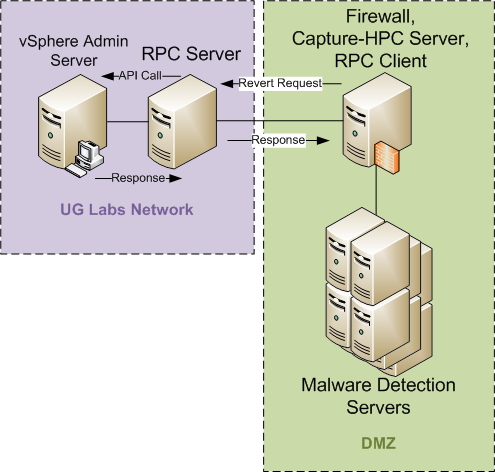
\includegraphics[width=0.8\textwidth]{img/revert-rpc.png}
\caption{Revert RPC Architecture}
\label{fig:revert-1}
\end{figure}

\subsubsection{Framework Integration}

Capture-HPC, being written in a combination of Java, C++ and C needs an
interface module before it can be integrated with the python framework.
Capture-HPC can be backed using a database for URLs, which is useful as it
allows us to build Capture-HPC's database format into a Django ORM which can
be used in the python code to access the database. Due to issues with the
version of Python on the locked-down Red Hat VM, most of the control happens
remotely, aided by the accessibility of the database server on the network. Each
Capture-HPC server has an RPC server and database server on it, which a remote
celery worker can connect to. Once the worker has loaded the URLs into the
database, it starts the Capture-HPC server and waits for the server to finish
processing URLs by periodically checking the database. Once the database
indicates all of the URLs have been scanned, the URLs are deleted from the
database and the RPC server is instructed to terminate the Capture-HPC server.
%TODO: DB stuff might be wrong
The results are returned by the celery worker to the framework for storage in
the framework's result storage database. Tasks for Capture-HPC are routed
specially through the framework, as only explicitly configured workers can
interface with the Capture-HPC server.

\subsubsection{Exclusion Lists}

The exclusion lists used to determine what activity is judged by the Capture-HPC
clients as malicious also needs to be maintained. The Capture-HPC server is
capable of sending the lists to the clients, allowing easy distribution of new
exclusion lists. The exclusion lists as of time of writing are included in
the attached data package, and are stored under the project version control, but the lists
created are only tested with Windows XP, so it is quite possible that they will
need to be modified for use under Windows 7 or Windows Vista.

